\subsection{Program master GBTx with external \itwoc adapter}
Before proceeding, for GBTx DB, follow the instructions on
\autoref{sec:hardware-ext-i2c} to configure the hardware;
for DCB, connect \itwoc adapter to the GBTx master FFC breakout board, or DCB
mainboard as described on \autoref{sec:dcb-master-i2c} or
\autoref{sec:dcb-data-i2c}.

All GBTx configuration files are publicly available at
\url{https://github.com/ypsun-umd/gbtx_communication_doc/releases}.
Always use latest release.

It is recommended to use the latest version of \textbf{GBTX programmer} provided by
CERN\footnote{
    Latest release can be found in CERN gitlab:
    \url{https://gitlab.cern.ch/gbtproj/gbtxprogrammer/tree/master/releases}.
    CERN credential needed to access the content.
}.

\begin{figure}[!ht]
    \centering
    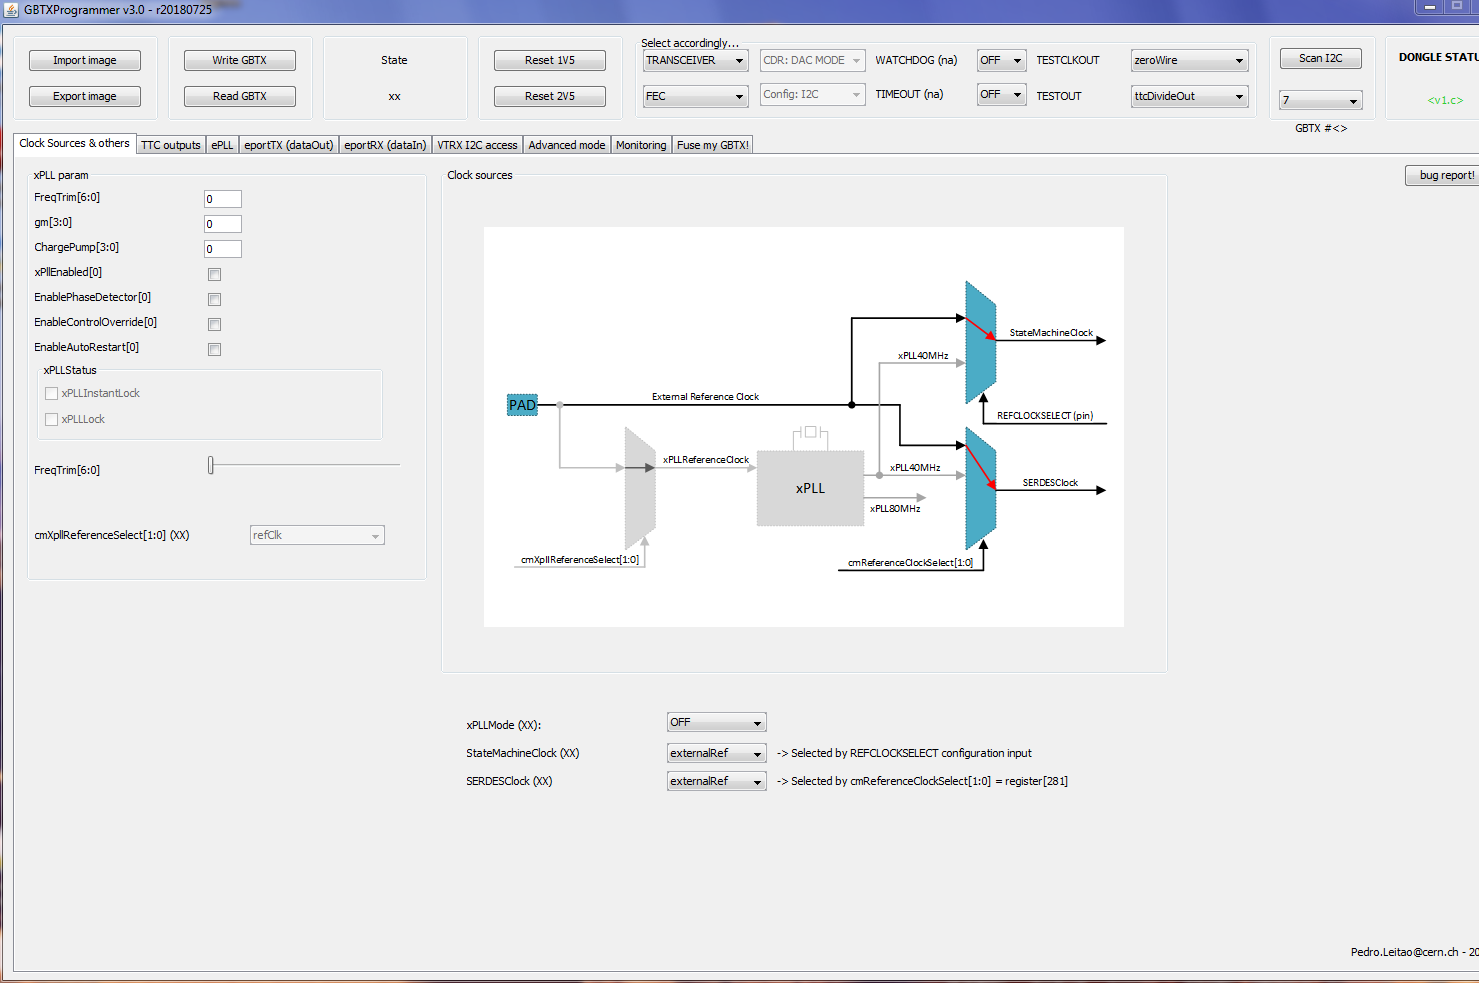
\includegraphics[width=0.9\textwidth]{res/gbtx_programmer_v3_ui.png}
    \caption{Main UI of GBTX programmer, version 3.}
    \label{fig:gbtx-programmer-ui}
\end{figure}

Click \textbf{Import image} and load a configuration file, then click
\textbf{Write GBTX} to write to master GBTx via \itwoc.

\begin{leftbar}
    During DCB pilot testing, at least one DCB could not be programmed by the
    latest version of GBTX Programer: It would get stuck in state 10.
    In that case, please revert back to GBTX Programer v1.
\end{leftbar}

\begin{figure}[!ht]
    \centering
    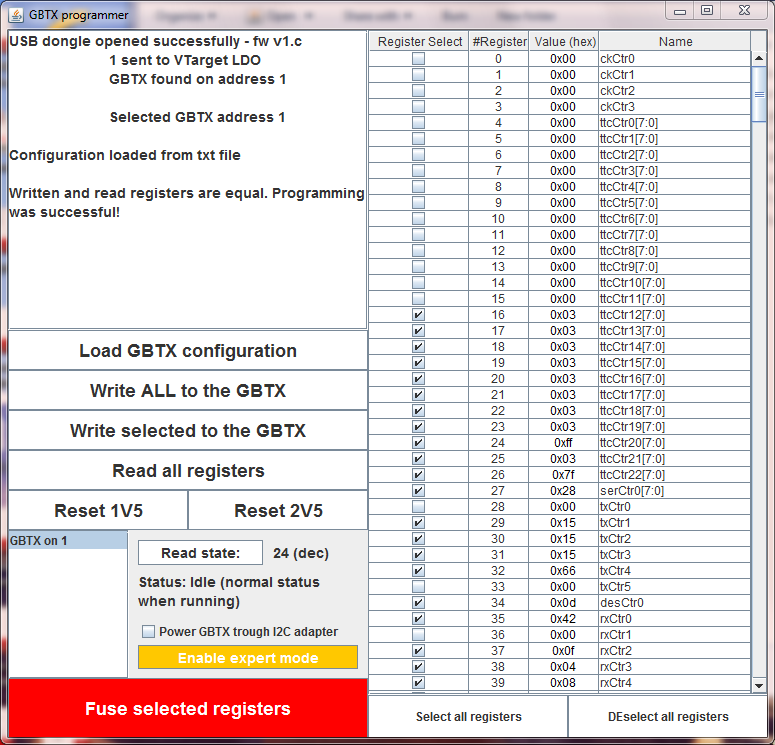
\includegraphics[width=0.9\textwidth]{res/gbtx_programmer_v1_ui.png}
    \caption{Main UI of GBTX programmer, version 1.}
    \label{fig:gbtx-programmer-ui}
\end{figure}

Launch the programmer, a typical UI is shown in
\autoref{fig:gbtx-programmer-ui},
Click \textbf{Load GBTX configuration} and load a configuration file, which is

Then click \textbf{Write ALL to the GBTX}. Check the returned message to make
sure everything works (supposedly).
Now click \textbf{Read state}.
If the master GBTx is configured correctly and is connected to a working
MiniDAQ, the return value should be:

\begin{lstlisting}
24 (dec): Idle (normal status when running)
\end{lstlisting}
